\documentclass[11pt]{article}
\usepackage[margin=1in]{geometry}
\usepackage{graphicx}
\usepackage{amsmath}
\usepackage{float}
\usepackage{setspace}
\setstretch{1.05}

\title{Internal Specification-Sensitivity Analysis of the Water Scarcity--GDP Growth Estimate}
\author{Draft for ECN 726 Term Project}
\date{\today}

\begin{document}
\maketitle

\begin{abstract}
This paper revisits the headline GDP-growth estimate in Frost, Madeira, and Martinez Jaramillo (2025) by conducting an internal specification-sensitivity analysis over 120 alternative specifications, varying functional form and estimator choice. The replicated baseline coefficient on freshwater withdrawal as a share of available freshwater is $-0.102$. Across the 120-specification grid, 85.8\% of estimates are negative, with a mean of $-0.292$ and a median of $-0.144$, indicating that the direction of the scarcity--growth association is consistent across most modeling choices. However, only 29.2\% of specifications reach statistical significance at the 5\% level, and the magnitude varies substantially. A meta-regression reveals that nonlinear functional forms---particularly the interaction of scarcity with income---produce the largest shifts in the coefficient, while the between estimator reverses its sign, suggesting that cross-country confounders inflate the cross-sectional association. These findings indicate that the original baseline is a conservative estimate whose sign is directionally stable but whose precision and magnitude depend on assumptions about functional form and the source of identifying variation.
\end{abstract}

\section{Introduction}

Water scarcity is an increasingly important constraint on economic activity. Frost, Madeira, and Martinez Jaramillo (2025) investigate whether this constraint has macroeconomically relevant effects, estimating the association between freshwater withdrawal intensity and GDP growth, investment, and inflation across a panel of 169 countries. Their headline finding is that water scarcity---measured as freshwater withdrawal as a share of available freshwater---is negatively and significantly associated with GDP growth, with a coefficient of $-0.102$ (Table 3, column 3, p.\ 15). This estimate implies that each additional percentage point of scarcity is associated with roughly 0.10 percentage points of lower annual growth.

The focal metric of this study is that coefficient. Using the replicated Stata workflow, I exactly reproduce the baseline in the 1990--2020 panel: $\hat{\beta} = -0.102$ with a standard error of 0.039 ($N = 4{,}583$). However, a single point estimate obscures the sensitivity of the result to the many modeling decisions embedded in its construction---the choice of functional form, the scarcity measure's denominator, the panel-data estimator, and the treatment of distributional heterogeneity. Any one of these decisions could shift the estimate substantially.

To assess this sensitivity, I conduct an internal specification-sensitivity analysis following the approach proposed by Banzhaf and Smith (2007). I systematically vary two primary dimensions of modeling choice---functional form (5 alternatives) and estimator (8 alternatives)---crossed with the authors' three scarcity measures, producing a grid of 120 specifications. Each specification yields an estimate of the scarcity--growth coefficient, and the full distribution is summarized by a specification curve and a meta-regression that decomposes the variation into contributions from each modeling decision.

Three findings emerge. First, the direction of the association is consistent: 85.8\% of the 120 estimates are negative, indicating sign stability across the specification space. Second, the magnitude and statistical significance are sensitive: only 29.2\% of specifications reach significance at the 5\% level, and the point estimate ranges from mildly positive (under the between estimator) to several times larger than the baseline (under nonlinear forms). Third, functional form is the most consequential modeling choice: specifications that allow the scarcity--growth gradient to interact with income produce the largest shifts, suggesting the linear baseline may understate the drag for lower-income economies.

\section{Data}

The extension reuses the replication package data pipeline, merging four formatted panel sources: World Bank macroeconomic indicators (GDP growth, gross fixed capital formation, CPI inflation), Aquastat water data from the Food and Agriculture Organization (freshwater withdrawal volumes and renewable resource estimates), Worldwide Governance Indicators, and Penn World Table series (real GDP at PPP). The merged panel is unbalanced and spans 169 countries over the period 1990--2020, yielding approximately 4,583 country-year observations for the baseline GDP growth regression.\footnote{The original paper reports $N = 4,583$ for Table 3, column (3). My Python replication matches this count exactly for the available-freshwater specification. Slight differences across scarcity measures arise because not all countries report all three denominators in every year.}

\subsection*{Variable definitions}

The dependent variable is annual real GDP growth, expressed in percentage points. The baseline regressors are:

\begin{itemize}
    \item \textit{Water use}: log total freshwater withdrawal per capita (in annual cubic meters), measuring the volume of water used across all sectors of the economy.
    \item \textit{Water scarcity}: freshwater withdrawal as a share of available resources. Three alternative denominators define three measures: (i) internal renewable resources (domestically generated river flows and groundwater recharge), (ii) total renewable resources (internal plus transboundary inflows), and (iii) available freshwater (total renewable resources adjusted for environmental water requirements). The third measure is the authors' preferred specification.
    \item \textit{Income}: log GDP per capita at purchasing power parity (2017 USD), serving as a proxy for development level and institutional quality.
\end{itemize}

Consistent with the original code, each scarcity measure is capped at 100 percent and winsorized at the top percentile before entering the regression. Values above 100\% are physically meaningful (they arise from non-renewable aquifer extraction or desalination), but the authors cap them to limit the influence of extreme outliers.

\subsection*{Summary statistics}

Table~\ref{tab:sumstats} reports summary statistics for the key variables, drawn from Table 2 of the original paper. The median scarcity ratios are modest (7--12\%), but the means are substantially higher (21--28\%), reflecting a right-skewed distribution with a long tail of water-stressed countries. The standard deviations of the scarcity measures (29--33 percentage points) exceed their means, confirming large cross-country heterogeneity. GDP growth averages 4\% with a standard deviation of 6 percentage points, typical for a global panel that includes both stable advanced economies and volatile developing economies.

\begin{table}[H]
\centering
\caption{Summary statistics of key variables (1990--2020, 169 countries)}
\label{tab:sumstats}
\small
\begin{tabular}{lccccc}
\hline
Variable & Min & Median & Mean & Max & SD \\
\hline
Annual GDP growth (\%) & $-64$ & 4 & 4 & 150 & 6 \\
\hline
\multicolumn{6}{l}{\textit{Water scarcity (freshwater withdrawal as \% of):}} \\
\quad Internal resources & 0 & 10 & 26 & 100 & 33 \\
\quad Total renewable resources & 0 & 7 & 21 & 100 & 29 \\
\quad Available freshwater & 0 & 12 & 28 & 100 & 33 \\
\hline
\multicolumn{6}{l}{\textit{Controls (in logarithm):}} \\
\quad Total water withdrawal per capita & 2.0 & 5.8 & 5.6 & 7.8 & 1.2 \\
\quad GDP per capita (PPP, 2017 USD) & 6.1 & 9.2 & 9.1 & 11.7 & 1.2 \\
\hline
\end{tabular}
\par\medskip
\footnotesize\textit{Notes}: Statistics reproduced from Table 2 of Frost, Madeira, and Martinez Jaramillo (2025). Scarcity measures are capped at 100\% and winsorized at the top percentile. Log GDP per capita ranges from approximately USD 445 to USD 120,571 in levels.
\end{table}

\subsection*{Measurement caveats}

Two features of the data merit attention. First, Aquastat water data are collected at irregular intervals (typically every five years) and interpolated or carried forward to fill annual gaps. The ``annual'' variation in scarcity within a country is therefore smoother than the annual variation in GDP growth, which could attenuate the within-country signal that the fixed-effects estimator relies on. Second, country-level aggregation masks substantial subnational heterogeneity in water availability---a concern the original authors acknowledge for the Americas region but do not address econometrically. Both issues bias against finding a significant scarcity effect, suggesting the estimates may represent a lower bound on the true relationship.

\section{Model Specification}

The original paper motivates the empirical analysis with a modified Cobb-Douglas production function in which water enters as an additional factor of production. Output for country $c$ in year $t$ is:
\begin{equation}
Y_{ct} = TFP_{ct} \cdot \bigl[g(W_{ct}, WS_{ct})\bigr]^{1-\alpha-\theta} \cdot \bigl[K_{ct}^{p}(W_{ct})\bigr]^{\alpha} \cdot \bigl[L_{ct} \cdot h(W_{ct})\bigr]^{\theta},
\label{eq:cobb_douglas}
\end{equation}
where $W_{ct}$ is water withdrawal, $WS_{ct}$ is water scarcity, and $g(\cdot)$ captures the effective productivity contribution of water. The authors parameterize this as:
\begin{equation}
g(W_{ct}, WS_{ct}) = \frac{W_{ct}}{1 + WS_{ct}},
\label{eq:g_function}
\end{equation}
so that higher scarcity lowers the effective water input through a factor proportional to $1/(1+WS_{ct})$.

Taking logarithms of (\ref{eq:cobb_douglas}) yields a linear expression in which log output depends additively on log TFP, log capital, log labor, log water use, and a negative term in $\ln(1+WS_{ct})$. The empirical specification replaces this structural object with a linear panel-data approximation:
\begin{equation}
Y_{ct} = \beta_1 \ln(W_{ct}^{pc}) + \beta_2 \, WS_{ct} + \beta_3 \ln(GDP_{ct}^{pc}) + \alpha_c + \alpha_t + \varepsilon_{ct},
\label{eq:panel}
\end{equation}
where $Y_{ct}$ is annual GDP growth, $W_{ct}^{pc}$ is total water withdrawal per capita, $WS_{ct}$ is one of the three scarcity measures, $GDP_{ct}^{pc}$ is GDP per capita at PPP, $\alpha_c$ and $\alpha_t$ are country and year fixed effects, and $\varepsilon_{ct}$ is the error term. Standard errors are clustered by country to allow for arbitrary within-country serial correlation.

Two features of this specification deserve comment. First, the transition from the structural model to the estimating equation is approximate: the log-linearization of (\ref{eq:cobb_douglas}) would produce $\ln(W_{ct})$ and $-\ln(1+WS_{ct})$ rather than the linear scarcity ratio $WS_{ct}$ that enters (\ref{eq:panel}). A first-order Taylor expansion of $\ln(1+WS)$ around zero justifies the linear approximation when scarcity is small, but the approximation deteriorates for high-scarcity countries---a point that motivates the nonlinear functional forms tested in the extension. Second, log GDP per capita serves as a proxy for the combined effects of TFP, capital intensity, and labor quality, which are not separately observed at annual frequency for the full 169-country panel.

The identifying assumption is strict exogeneity of the water variables conditional on fixed effects. Country effects absorb time-invariant confounders (geography, baseline institutions, resource endowments), and year effects absorb global shocks (commodity cycles, pandemic effects). However, this strategy cannot rule out two threats. Reverse causality arises if weak economic growth reduces water demand or shifts sectoral composition in ways that lower measured scarcity, generating a spurious negative association. Omitted time-varying confounders---changes in trade policy, energy infrastructure, or governance quality---may jointly drive both growth and water withdrawal. The authors acknowledge these concerns (footnote 8 of the original paper) and do not claim causality. This extension maintains that framing and evaluates the stability of the association across plausible modeling alternatives.

\section{Analysis Design}

To evaluate the fragility of the baseline estimate, I construct a 120-specification grid defined by the Cartesian product of three dimensions: 3 scarcity measures $\times$ 5 functional forms $\times$ 8 estimators = 120 specifications. Following Banzhaf and Smith (2007), the resulting estimates are collected into a specification curve and summarized by a meta-regression that identifies which modeling decisions systematically shift the scarcity--growth coefficient.

\paragraph*{Scarcity measure}

The first dimension varies the denominator of the scarcity ratio: internal renewable resources, total renewable resources, or available freshwater. These three measures are highly correlated (85--95\%, per Table A.2 of the original paper) but differ in scope. Internal resources count only domestically generated flows; total renewable resources add transboundary inflows; available freshwater further adjusts for environmental water requirements. The authors report all three in Table 3 but never test whether the choice of denominator drives the result. Including all three in the grid directly tests this.

\paragraph*{Functional form}

The second dimension varies the parametric relationship between scarcity and growth. Five specifications are tested, each motivated by a specific economic hypothesis.

\textit{Linear (baseline).} This replicates the authors' original specification in Equation (3). It serves as the anchor against which all other forms are compared.

\textit{Quadratic.} The authors' own quantile results (Table A.4) show that the scarcity coefficient is most negative at the 25th percentile of the growth distribution and least negative at the 75th percentile. If the true relationship is convex---meaning the marginal drag from scarcity accelerates at higher scarcity levels---then a linear specification underestimates the effect for high-scarcity countries and overestimates it for low-scarcity countries. Adding a squared scarcity term directly tests for this curvature.

\textit{Scarcity $\times$ log GDP per capita interaction.} The paper's theoretical model (Equation 1) treats water as complementary with TFP, capital, and labor, all of which correlate with national income. Richer countries may buffer the productivity drag of scarcity through more efficient infrastructure, better water pricing (as discussed in the paper's Section 5), or a sectoral shift away from water-intensive agriculture. This interaction tests whether development level moderates the scarcity--growth relationship, which has direct policy implications for whether the pooled estimate applies equally to advanced and developing economies.

\textit{Scarcity $\times$ log water use per capita interaction.} The baseline specification includes water use and water scarcity as separate additive regressors but never allows them to interact. A country that withdraws a large share of its available resources \textit{and} uses a large volume of water per capita (e.g., an agricultural economy with heavy irrigation) faces a fundamentally different constraint than a country with high scarcity but low absolute use (e.g., an arid country with limited economic activity). This interaction tests whether the growth penalty from scarcity is amplified when absolute water demand is also high.

\textit{Piecewise threshold at median scarcity.} The authors' functional form $g(W, WS) = W/(1+WS)$ imposes smooth, monotonic decay in the productivity contribution of water. However, production theory suggests that inputs may become binding constraints only beyond certain thresholds---a country at 5\% scarcity may face no meaningful growth drag, while a country at 50\% may face an acute bottleneck. The piecewise specification allows the slope of the scarcity--growth relationship to change at the sample median, testing for such a discontinuity.

\paragraph*{Estimator choice}

The third dimension varies the panel-data estimator. Eight estimators are tested, each probing a distinct aspect of the data structure or identifying assumption.

\textit{Country FE only (no year effects).} The baseline includes both country and year fixed effects. Year effects absorb global shocks common to all countries---commodity price cycles, global recessions, and pandemic effects. Dropping year effects tests whether these global trends are confounding the scarcity--growth relationship. If the coefficient changes substantially, the baseline result depends in part on controlling for common time shocks.

\textit{Two-way FE (country + year).} This is the authors' baseline estimator. It absorbs all time-invariant country heterogeneity and all country-invariant time shocks, identifying the scarcity effect from within-country deviations around country means, purged of global trends.

\textit{Random effects.} The fixed-effects estimator discards all between-country variation, which is where most of the scarcity variation lies (Table 2 of the original paper shows enormous cross-country dispersion in scarcity ratios). The random-effects estimator uses both within- and between-country variation, under the assumption that country-specific effects are uncorrelated with the regressors. A Hausman test comparing RE to FE indicates whether the between-country variation is informative or contaminated by omitted variables.

\textit{Between estimator.} This isolates purely cross-country variation by regressing country means of growth on country means of scarcity. If the scarcity--growth relationship operates primarily through long-run structural differences (e.g., permanently water-scarce countries developing along different growth paths), the between estimator should reveal a strong effect. If it attenuates or reverses, this suggests the cross-sectional correlation is driven by confounders that the within estimator purges.

\textit{First-differenced OLS.} An alternative to fixed effects that eliminates country-specific intercepts by differencing consecutive observations rather than demeaning. Under strict exogeneity, both FE and FD are consistent, but they differ in efficiency depending on the error structure: FD is more efficient if errors follow a random walk, while FE is more efficient if errors are serially uncorrelated (Wooldridge, 2010). Comparing FD to FE provides a diagnostic for the serial correlation properties of the residuals.

\textit{Panel quantile at Q25, Q50, Q75.} The Machado and Santos Silva (2019) panel quantile estimator with country fixed effects allows the scarcity coefficient to vary across the conditional distribution of GDP growth. The authors' Table A.4 already documents that the effect is strongest at Q25. Re-estimating across functional forms tests whether this tail-risk pattern persists under nonlinear specifications. As noted by the authors, this estimator is applied without year fixed effects because it is inconsistent with ancillary parameters such as year dummies (Machado and Santos Silva, 2019).

\paragraph*{Meta-regression}

The distribution of the 120 estimates is summarized via a meta-regression:
\[
\begin{aligned}
\hat{\beta}_s =\ & \gamma_0 + \gamma_1 d_{quadratic,s} + \gamma_2 d_{income,s} + \gamma_3 d_{use,s} + \gamma_4 d_{threshold,s} + \gamma_5 d_{internal,s} + \gamma_6 d_{renewable,s} \\
& + \gamma_7 d_{countryFE,s} + \gamma_8 d_{RE,s} + \gamma_9 d_{between,s} + \gamma_{10} d_{FD,s} + \gamma_{11} d_{Q25,s} + \gamma_{12} d_{Q50,s} + \gamma_{13} d_{Q75,s} + \varepsilon_s,
\end{aligned}
\]
where the omitted baseline category encompasses the linear functional form, the available-freshwater scarcity measure, and the two-way fixed-effects estimator. The coefficients $\gamma_1$ through $\gamma_{13}$ measure the average shift in the scarcity--growth estimate attributable to each modeling decision, holding all others at their baseline values. Standard errors are heteroskedasticity-robust. Because all 120 specifications are estimated from the same underlying dataset, the meta-regression standard errors should be interpreted as descriptive summaries of the specification space rather than as formal inferential quantities.\footnote{This follows the practice in Banzhaf and Smith (2007), who estimate their meta-regression (Table VI) with simple OLS on estimates derived from the same dataset.}

\section{Analysis Results}

All 120 specifications converged successfully. Table~\ref{tab:dist} reports the summary distribution of the resulting scarcity coefficients, and Table~\ref{tab:meta} reports the meta-regression. The specification curve in Figure~\ref{fig:spec_curve} displays all 120 point estimates sorted by magnitude with 95\% confidence intervals, alongside a decision matrix indicating which modeling choices are active in each specification.

\subsection*{Distribution of estimates}

The average estimate across the grid is $-0.292$ and the median is $-0.144$. The interquartile range spans $-0.364$ to $-0.035$, covering strictly negative values. Overall, 85.8\% of the 120 estimates carry a negative sign. However, only 29.2\% are statistically significant at the 5\% level. This pattern indicates that while the \textit{direction} of the scarcity--growth association is consistent across the vast majority of specifications, the statistical precision of the estimate is sensitive to modeling choices. In particular, the magnitude of the coefficient varies by more than an order of magnitude across the grid, ranging from large negative values under nonlinear or lower-tail specifications to mildly positive values under the between estimator. The authors' baseline of $-0.102$ lies near the upper end of this distribution, suggesting it represents a relatively conservative point within the broader model space.

\begin{table}[htbp]
\centering
\caption{Distribution of the 120 scarcity estimates}
\label{tab:dist}
\small
\begin{tabular}{lc}
\hline
Statistic & Value \\\\
\hline
Successful specifications & 120 \\\\
Mean beta & -0.292 \\\\
Median beta & -0.144 \\\\
25th percentile & -0.364 \\\\
75th percentile & -0.035 \\\\
Share negative (\%) & 85.8 \\\\
Share significant at 5\% (\%) & 29.2 \\\\
\hline
\end{tabular}
\end{table}


\begin{figure}[H]
\centering
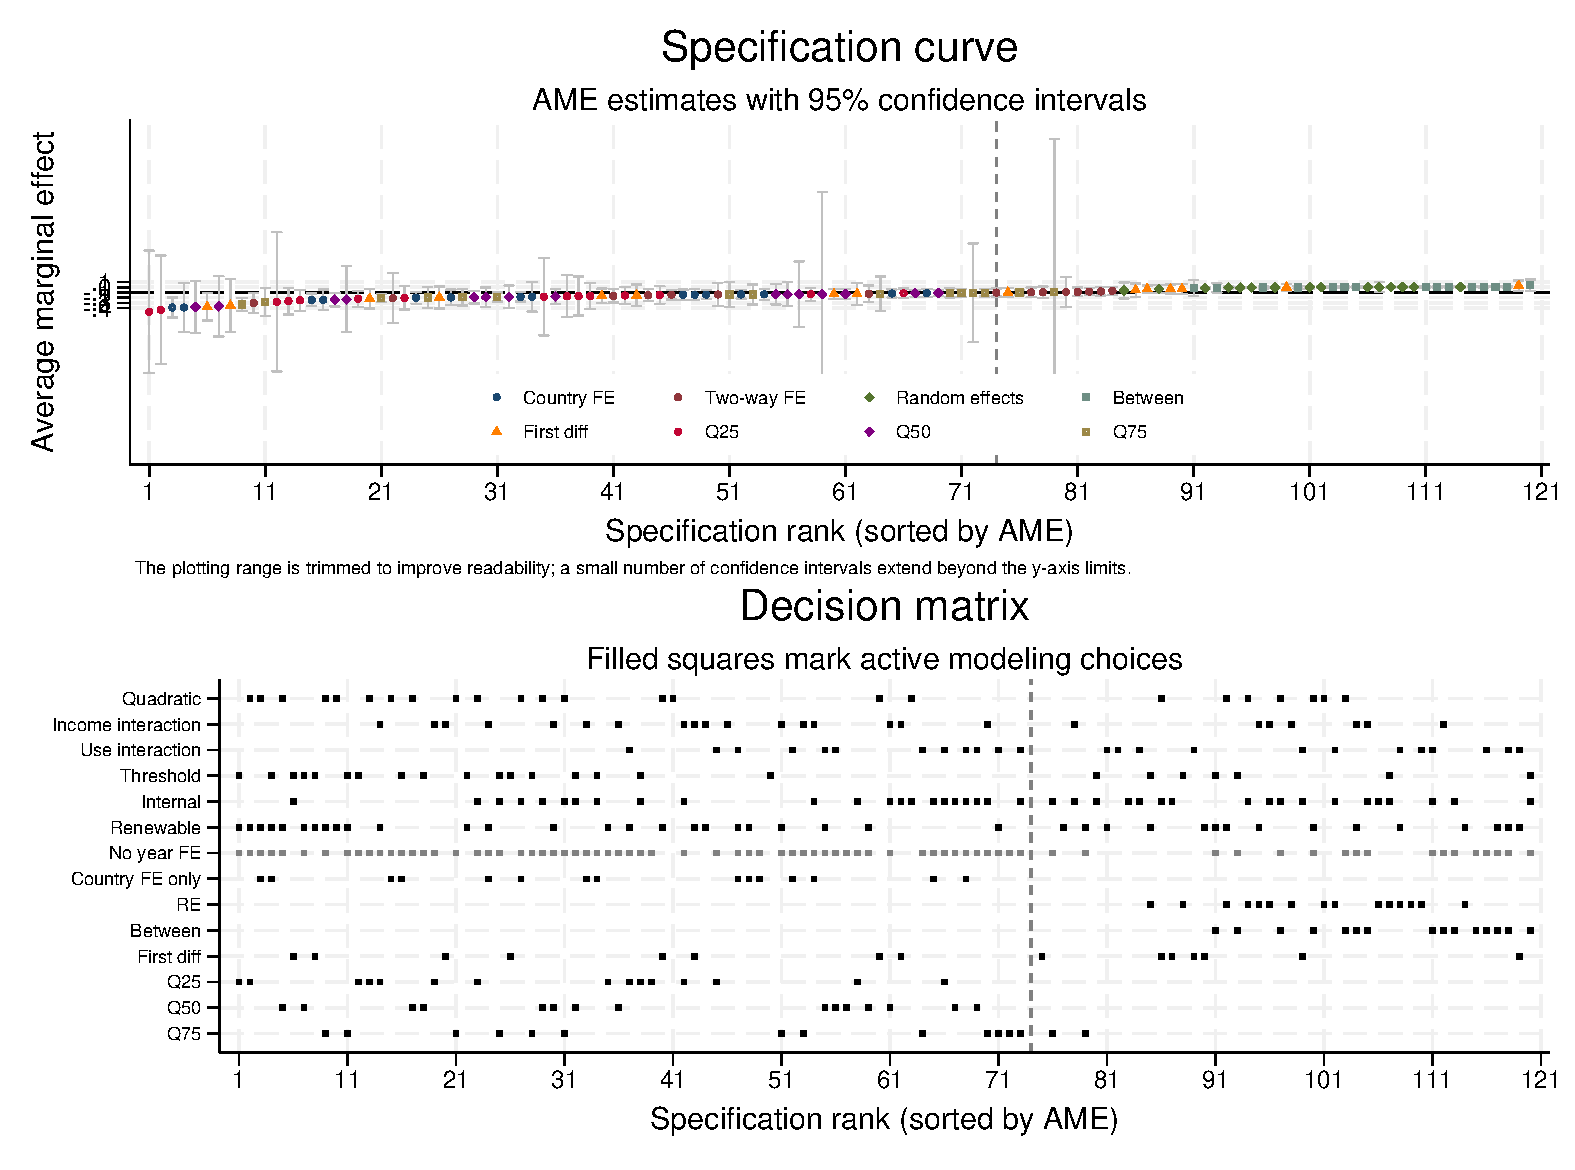
\includegraphics[width=\textwidth]{../figures/specification_curve.pdf}
\caption{Specification curve for the 120 water scarcity estimates. The upper panel plots point estimates sorted by magnitude with 95\% confidence intervals, color-coded by estimator. The dashed vertical line marks the authors' baseline ($-0.102$). The lower panel shows which modeling decisions are active for each specification.}
\label{fig:spec_curve}
\end{figure}

\subsection*{Meta-regression results}

\begin{table}[htbp]
\centering
\caption{Meta-regression of water scarcity estimates}
\label{tab:meta}
\small
\begin{tabular}{lcc}
\hline
Variable & Coefficient & Robust SE \\\\
\hline
Constant & -0.0059 & 0.0708 \\\\
Quadratic form & -0.1518 & 0.0503 \\\\
Scarcity x log GDP per capita & -0.7720 & 0.1480 \\\\
Scarcity x log water use & 0.1027 & 0.0838 \\\\
Threshold form & -0.2237 & 0.0433 \\\\
Internal scarcity measure & 0.0469 & 0.0771 \\\\
Renewable scarcity measure & -0.1166 & 0.0858 \\\\
Country FE only & -0.1196 & 0.0369 \\\\
Random effects & 0.1886 & 0.0741 \\\\
Between estimator & 0.2215 & 0.0809 \\\\
First differences & -0.3782 & 0.2432 \\\\
Quantile 0.25 & -0.1572 & 0.0403 \\\\
Quantile 0.50 & -0.1102 & 0.0393 \\\\
Quantile 0.75 & -0.0722 & 0.0574 \\\\
\hline
\multicolumn{3}{p{0.9\textwidth}}{\footnotesize Notes: OLS meta-regression with heteroskedasticity-robust standard errors. The omitted categories are the linear specification, the available-freshwater scarcity measure and the two-way fixed-effects estimator.}
\end{tabular}
\end{table}


The meta-regression decomposes the variation across the 120 estimates into contributions from each modeling decision. Three sets of findings emerge.

\textit{Functional form matters most.} Relative to the linear baseline, introducing a quadratic term shifts the average scarcity coefficient downward by $-0.152$, the threshold specification shifts it by $-0.224$, and the income interaction produces the largest shift at $-0.772$. These are economically substantial: the income interaction alone moves the estimated scarcity--growth gradient from near zero to roughly $-0.78$, suggesting that the linear specification may mask important heterogeneity in how scarcity affects growth across income levels. The water-use interaction, by contrast, produces a small and statistically insignificant upward shift of $0.103$, indicating that absolute water use does not meaningfully amplify the scarcity drag once the level of scarcity itself is controlled for.\footnote{At the 10th percentile of log GDP per capita ($\approx 7.0$, corresponding to roughly USD 1,100), the net marginal effect of scarcity ranges from $-0.325$ to $-0.194$ depending on the scarcity measure ($-0.271$ for the baseline available-freshwater measure). At the 90th percentile ($\approx 10.8$, corresponding to roughly USD 49,000), the effect is much smaller, ranging from $-0.049$ to $-0.025$. This indicates that water scarcity imposes a substantially larger growth penalty on poorer countries than on richer economies, likely because advanced countries have better infrastructure or less water-intensive production to buffer the constraint.}

\textit{Estimator choice reveals a between-within divergence.} Dropping year fixed effects (country FE only) makes the coefficient $-0.120$ more negative on average, confirming that global time trends partially offset the within-country scarcity signal in the two-way FE baseline. The random-effects estimator shifts the coefficient upward by $0.189$, and the between estimator shifts it upward by $0.222$. Added to the baseline constant of $-0.006$, the between estimator yields an average point estimate that is mildly \textit{positive}---a sign reversal, not merely an attenuation. This suggests that the cross-country correlation between scarcity and growth is dominated by confounders: countries with high scarcity (arid Middle Eastern and North African economies, for example) may also have high GDP per capita from resource wealth, generating a spurious positive cross-sectional association. The within-country FE estimator purges these time-invariant confounders, revealing the negative within-country signal. This divergence supports the use of fixed-effects estimation for this question.

The first-differences estimator produces a large downward shift of $-0.378$, though with a wide standard error ($0.243$). Since first differencing identifies the effect from year-to-year changes rather than deviations from long-run means, the larger FD coefficient may reflect the short-run impact of acute scarcity shocks (e.g., droughts) on growth, which could be more severe than the drag implied by sustained scarcity levels.

\textit{Quantile estimates confirm tail risk, with a caveat.} The Q25, Q50, and Q75 specifications shift the coefficient downward by $-0.157$, $-0.110$, and $-0.072$, respectively. The monotonic gradient confirms the original paper's finding that scarcity is most damaging during low-growth episodes, consistent with water scarcity acting as a constraint that binds most tightly when the economy is already weak. However, since the panel quantile estimator is applied without year fixed effects (as required by Machado and Santos Silva, 2019), part of this downward shift may reflect the omission of year effects rather than distributional heterogeneity per se---the country-FE-only estimator, which also drops year effects, shows a directionally similar shift of $-0.120$. The incremental contribution of the quantile specification beyond the missing-year-effects channel is therefore smaller than the raw coefficients suggest, on the order of $-0.04$ to $-0.05$ for Q25.

\textit{Scarcity measure matters less.} Switching from available freshwater to internal resources shifts the coefficient by $0.047$ (insignificant), and switching to total renewable resources shifts it by $-0.117$ (also imprecise). The three scarcity measures produce broadly similar estimates, consistent with their high correlation. This suggests the choice of denominator is not a major source of fragility in the baseline result, though the measures were not standardized prior to estimation and differ in scale, so these meta-regression coefficients should be interpreted with caution.

\section{Conclusions}

This internal specification-sensitivity analysis evaluates the stability of the water scarcity--GDP growth estimate in Frost, Madeira, and Martinez Jaramillo (2025) across 120 alternative specifications. Three findings emerge.

First, the direction of the association is consistent: 85.8\% of the 120 estimates are negative. Water scarcity, however measured, is associated with lower GDP growth in the vast majority of specifications. This directional stability holds across all three scarcity measures, all five functional forms, and most estimators.

Second, the magnitude of the estimate is highly sensitive to modeling choices. The meta-regression identifies functional form as the most consequential dimension. Specifications that allow the scarcity--growth gradient to vary with income level produce coefficients several times larger than the linear baseline, suggesting that the original estimate of $-0.102$ may understate the drag for lower-income economies where water infrastructure and sectoral buffers are weaker. Estimator choice is the second most influential dimension: the between estimator yields a positive cross-sectional association, while within-country fixed-effects and first-differences estimators produce negative coefficients, indicating that time-invariant confounders contaminate the cross-country signal.

Third, the quantile results support the interpretation that water scarcity poses a downside risk---the estimated drag is largest during low-growth episodes and smallest during high-growth episodes, though part of this pattern may reflect the omission of year fixed effects in the quantile estimator rather than pure distributional heterogeneity.

\subsection*{Limitations}

Several limitations should be kept in mind when interpreting these results. The identifying strategy relies on within-country variation conditional on fixed effects and cannot rule out reverse causality: weak economic growth may reduce water demand or alter sectoral composition in ways that lower measured scarcity, biasing the coefficient away from zero. Omitted time-varying confounders---such as changes in trade exposure, energy composition, or institutional quality---may also jointly determine growth and water withdrawal patterns.

On the data side, the Aquastat water series are collected at irregular intervals and interpolated to annual frequency, which smooths the within-country variation that the fixed-effects estimator exploits. This likely attenuates the estimated effect. Country-level aggregation further obscures subnational heterogeneity in water availability, limiting the applicability of these estimates to regional or local contexts.

Finally, the meta-regression treats 120 estimates derived from the same dataset as independent observations. While heteroskedasticity-robust standard errors are reported, the mechanical correlation among specifications sharing the same data means that the meta-regression $p$-values overstate inferential precision. The meta-regression coefficients are best interpreted as descriptive summaries of how the estimate moves across the specification space.

\subsection*{Next steps}

Several extensions would strengthen the analysis. First, the specification grid could be expanded along additional dimensions---notably sample composition (OECD versus non-OECD, continental subsets, excluding 2020) and additional controls (governance quality, trade openness, agricultural GDP share)---to test whether the sign stability documented here survives further perturbation. Second, the income-interaction result warrants deeper investigation: computing the net marginal effect of scarcity at different income levels using the underlying regression coefficients would clarify whether scarcity is primarily a drag on lower-income economies or whether the gradient is more uniform. Third, testing for cross-sectional dependence (e.g., via the Pesaran CD test) and estimating at least one specification with spatially robust standard errors (e.g., Driscoll-Kraay) would address the concern that regional climate patterns induce correlated errors across countries. Finally, identification strategies capable of isolating the causal effect of scarcity---such as instrumental variables based on exogenous rainfall variation or upstream dam construction---would move the analysis beyond the associational framework that both the original paper and this extension operate within.

\begin{thebibliography}{9}
\bibitem{banzhaf_smith_2007} Banzhaf, H. Spencer, and V. Kerry Smith. 2007. Meta-analysis in model implementation: Choice sets and the valuation of air quality improvements. \textit{Journal of Applied Econometrics} 22(6): 1013--1031.
\bibitem{frost_madeira_mj_2025} Frost, Jon, Carlos Madeira, and Serafin Martinez Jaramillo. 2025. The economics of water scarcity. BIS Working Papers No. 1314.
\bibitem{machado_santos_silva_2019} Machado, Jose A. F., and J. M. C. Santos Silva. 2019. Quantiles via moments. \textit{Journal of Econometrics} 213(1): 145--173.
\bibitem{wooldridge_2010} Wooldridge, Jeffrey M. 2010. \textit{Econometric Analysis
of Cross Section and Panel Data}. 2nd ed. Cambridge, MA: MIT Press.
\end{thebibliography}
\end{document}
